\tikzset{
	inner/.style = {circle, draw=black, fill=darkgray},
	leaf/.style = {circle}
}

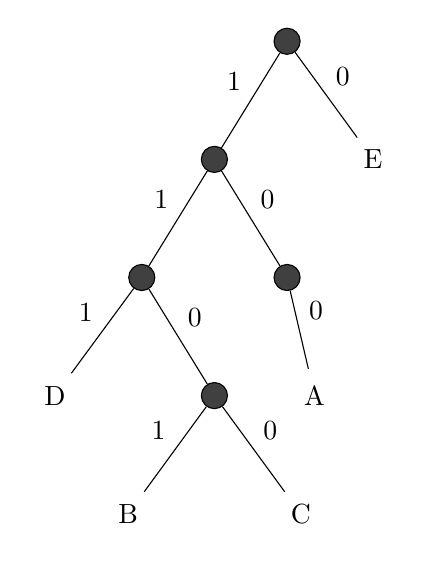
\begin{tikzpicture}
	\tikzstyle{every node}=[]
	\node[inner]{}
		child {
			node[inner,left]{}
			child {
				node[inner,left]{}
				child {
					node[leaf,left]{D}
					edge from parent node [above left] {1}
				}
				child {
					node[inner,right]{}
					child {
						node[leaf,left]{B}
						edge from parent node [above left] {1}
					}
					child {
						node[leaf,right]{C}
						edge from parent node [above right] {0}
					}
					edge from parent node [above right] {0}
				}
				edge from parent node [above left] {1}
			}
			child {
				node[inner,right]{}
				child {
					node[leaf,right]{A}
					edge from parent node [above right] {0}
				}
				edge from parent node [above right] {0}
			}
			edge from parent node [above left] {1}
		}
		child {
			node[leaf,right]{E}
			edge from parent node [above right] {0}
		}
	;
\end{tikzpicture}
